\setlength{\footskip}{8mm}

\chapter{Incremental Behavior Modeling and Suspicious 
Activity Detection}
\label{ch:incremental}

\textit{We propose and evaluate an efficient method for automatic 
identification of suspicious behavior in video surveillance data that
incrementally learns scene-specific statistical models of human
behavior without requiring storage of large databases of training
data. The approach begins by building an initial set of models
explaining the behaviors occurring in a small bootstrap data set. The
bootstrap procedure partitions the bootstrap set into clusters then
assigns new observation sequences to clusters based on statistical
tests of HMM log likelihood scores. Cluster-specific likelihood
thresholds are learned rather than set arbitrarily. After
bootstrapping, each new sequence is used to incrementally update the
sufficient statistics of the HMM it is assigned to. In an evaluation
on a real-world testbed video surveillance data set, we find that
within one week of observation, the incremental method's false alarm
rate drops below that of a batch method on the same data. The
incremental method obtains a false alarm rate of 2.2\% at a 91\% hit
rate. The method is thus a practical and effective solution to the
problem of inducing scene-specific statistical models useful for
bringing suspicious behavior to the attention of human security
personnel.}

\section{Introduction}
\label{incremental-intro}

Human monitoring of video surveillance channels is increasingly
ineffective as the number of channels increases.  \textit{Anomaly
detection} aims to alleviate this problem by filtering out typical
events and only bringing suspicious events to the attention of human
security personnel.

We propose a new incremental method for learning behavior models and
detecting anomalies using hidden Markov model (HMM)-based clustering
on a small bootstrap set of sequences labeled as normal or suspicious.
After bootstrapping, we assign new observation sequences to behavior
clusters using statistical tests on the log likelihood of the sequence
according to the corresponding HMMs.  We label a sequence as
suspicious if it maps to an existing model of suspicious behavior or
does not map to any existing model.  After labeling, we either
incrementally update the sufficient statistics for the most likely
HMM's parameters or create a new HMM for the new sequence.

In an evaluation on a real-world video surveillance situation, we find
that the method is very effective at identifying suspicious
behavior. A batch method achieves a false positive rate of 8.6\% at a
100\% hit rate. The incremental method decreases the false alarm rate
to 2.2\% at a 91\% hit rate, and detection threshold tuning can
achieve an equal error rate of 95.8\% or a false alarm rate of 3.7\%
at a 100\% hit rate.  The experimental results demonstrate that our
incremental method is better able to learn new forms of normal
behavior, leading in turn to more effective anomaly detection. The
method is thus a practical and effective solution to the problem of
inducing scene-specific statistical models useful for bringing
suspicious behavior to the attention of human security personnel.

\section{Related Work}
\label{incremental-related-work}

In this section, we explore methods for incremental learning of
behavior models and active detection of anomalous deviations from the
learned typical behavior.  We build upon previous research in human
behavior
understanding \shortcite{davis98activity,masoud03recognition,cao04motion,sminchisescu05motion,li06behavior,du06activity,wang06gesture},
the use of dynamic graphical models such as hidden Markov models
(HMMs) and conditional random fields (CRFs) for behavior understanding
in specific
scenarios \shortcite{yamato92hmm,gao04dining,xiang05profiling,sminchisescu05motion,vail07activity},
and classification of behavior in videos to a priori known categories
\shortcite{nair02surveillance,lee03modeling,wu05behavior,arsic07behavior}.

Several research groups have investigated methods for video clustering
\shortcite{sakoe78dtw,zhong04detection,xiang05profiling,hautamaki08clustering,xiang08clustering,swears08clustering,xiang08modeling}. Especially effective are those methods using HMMs
to model different classes of behavior in video surveillance
data \shortcite{xiang05profiling,swears08clustering,xiang08modeling}.

There has been some work on anomalous time series detection outside
the context of video surveillance using relatively simple statistical
models \shortcite{turner10detection,yao10detection}.  However, these
methods learn single comprehensive models without addressing the
special requirement in video surveillance to capture an extremely wide
variety of typical behaviors.  This requires construction of a
collection of statistical models.  Intrusion detection requires
similar diversity in the statistical models.  Some of the work uses
ensembles of classifiers \shortcite{rasoulifard08incremental}, but
most of the research has focused on anomaly detection methods using
incremental
clustering \shortcite{burbeck04adwice,burbeck07incremental,ren08incremental,zhong08incremental,ekman08incremental}.
All of these methods generally work by comparing a new pattern against
a collection of clusters representing historically typical behavior
and classifying the new pattern as an anomaly if its distance from the
nearest cluster is above threshold.  We take a similar approach, with
a specific approach to clustering, distance measurement, and threshold
learning specific to the case of surveillance video.

Some incremental learning approaches have been applied to human
behavior modeling. \shortciteA{vasquez09incremental} incrementally
model vehicle and pedestrian trajectories using growing hidden Markov
models (GHMMs). The method builds a topological map and corresponding
GHMM using an incremental variant of the Baum-Welch algorithm. For
each new node in the map, a corresponding state and connectivity are
added to the GHMM. \shortciteA{kulic10incremental} model movement
primitives using HMMs and piece the primitives together with a higher
level HMM. Similar to Vasquez et al., the method incrementally adds
new hidden states when a new primitive model is built.

Besides human behavior modeling, \shortciteA{stenger01topology} first
propose the incremental Baum-Welch (IBW) algorithm on continuous
observations for background modeling. This algorithm is a
straight-forward adaptation of the original Baum-Welch algorithm to
incremental learning. They update the parameters by taking into
account the sufficient statistics. Although they use a single
observation sequence to update the parameters, but the sufficient
statistics still can represent the information computed for all of the
observed data. Later, \shortciteA{larrahondo05incremental} adapt this
algorithm to model discrete
observations. \shortciteA{cavalin08incremental} use the ensemble
training (ET) algorithm \shortcite{mackay97hmm} to the incremental
learning problem in alphanumeric character recognition. This algorithm
has never been used in incremental learning setting. The authors claim
that it is easy to adapt to this kind of setting since the parameters
of the final HMM are computed for each observation sequence
independently.

The existing work most similar to ours is the incremental learning
approach of \shortciteA{xiang08incremental}, who also model activity
in a scene incrementally after initialization from a small bootstrap
dataset. They build explicit probabilistic models of normal and
abnormal activity patterns in the bootstrap set then classify new
observations using a likelihood ratio test.  The models are global
joint models over the entire scene.  It is not clear how the
likelihood ratio test could handle completely new anomalous events
with low likelihoods under both models, and it is not clear whether a
global model is appropriate for detecting isolated anomalous behavior
in a scene.

Our method does not require an a priori model of anomalous human
behavior. It constructs an ensemble of simple models, adding to the
ensemble when the existing set is insufficient to represent new
cases. We associate each new observation with an individual model
using separate statistical tests on the observation's likelihood
according to each individual model.  Rather than globally modeling the
entire scene, our method takes a more local approach, separately
analyzing each individual moving object's behavior.  In an
experimental comparison of the two methods, we find statistical
testing of the likelihood to be superior to likelihood ratio tests,
and we find the local representation to be superior to the global
representation.

%A preliminary report on our clustering method appeared in a conference
%paper \shortcite{kan10clustering}, but it was limited to tracking only
%one human in a scene.  In this chapter, we have extended the work to
%include multiple human tracking, anomaly detection, and incremental
%learning.

The main contribution of the work described in this chapter is a new
modeling method for detection of anomalous events in surveillance
video based on simply-structured models and incremental learning that
is demonstrably able to evolve the models over time to adapt to new
behavior and also outperforms current techniques on the same data set.

\section{Behavior Model Bootstrapping}
\label{sec:incremental-bootstrap}

Simply-structured statistical models cannot hope to capture the
diversity of ``normal'' behavior in a given scene --- multiple models
are required.  However, it is difficult to determine how many and what
activities will occur in a scene a priori or based on manual
monitoring.  We therefore propose a method to automatically determine,
from a small bootstrap set, the common similar behaviors occurring in
a scene. The entire process of the method used in this section is
previously described in Section \ref{sec:batch-modeling} including
blob extraction, appearance-based blob tracking, blob feature vector
discretization, and behavior clustering.

This process results in a set of $K$ different typical behavior
clusters ${\cal C} = \{ c_1, c_2, \ldots, c_K \}$ with a set of $K$
corresponding HMMs ${\cal M} = \{ M_1, M_2, \ldots, M_K \}$.

\section{Anomaly Detection}
\label{incremental-detection}

We classify new sequences as abnormal if the most likely HMM for the
input sequence is associated with one of the abnormal
models, \textit{or} the $z$-scored per-observation log likelihood of
the sequence under that most likely model is less than a global
empirically determined threshold $\theta_z$. We previously described
this method in Section~\ref{sec:batch-anomaly-detection}.

One problem with this approach is that it never learns any new typical
behavior over time.  Given a small bootstrap set, the method may work
well for a short period of time, but as typical behavior evolves and
becomes more diverse, the false alarm rate may increase.

The naive solution to this problem is to retain all of the observation
data and retrain the system periodically.  However, this would require
storing all of the incoming data, requiring too much disk space. For
lifelong anomaly detection, we need a more adaptive approach that
learns new behaviors over time but does not require storing all of the
historical data. We solve this problem in the next section.

\section{Incremental Behavior Modeling for Anomaly Detection}
\label{incremental-inc-modeling}

In this section, we extend the basic anomaly detection method
previously described in Section~\ref{incremental-detection} using the
incremental maximum likelihood (IML) algorithm for HMMs
\shortcite{gotoh96incremental}. The incremental expectation maximization (EM)
procedure was originally proposed by \shortciteA{neal93em}. The basic
idea is to update the sufficient statistics for the parameters of the
HMMs as new events occur. In our approach, given an initial set of
observation sequence clusters and corresponding HMMs modeling the
behavior in the scene, when a new observation sequence arrives, we
first determine which cluster it falls into by performing statistical
tests on the sequence's likelihood according to each HMM model. Since
likelihood scores for different HMMs cannot be compared directly, we
select the most likely model based on the same $z$-scored
per-observation log likelihood measure introduced in
Section~\ref{sec:clustering-behavior-clustering} for the initial
behavior model clustering.

When the most likely model for a new observation sequence is a model
for a cluster of atypical behaviors, or when the new observation
sequence's likelihood according to the most likely model is not
sufficiently high, we raise an alert. If the operator gives feedback
that a new observation sequence marked as suspicious by the system is
in fact not suspicious, we create a new typical behavior cluster and
corresponding HMM for the false alarm sequence. If the likelihood
according to the most likely model is sufficiently high for one of the
pre-existing models and the operator confirms that the classification
is correct, we incrementally update the sufficient statistics for that
model; otherwise, we start a new cluster for the sequence, build a new
HMM for the new cluster, and label it according to the operator
feedback. This approach allows the system to raise alerts when unusual
behaviors are detected while adapting to gradual changes in behavior
patterns over time. The method is detailed in Algorithm
\ref{anomaly-detection-with-iml-algorithm}.

\begin{algorithm}
  \caption{Anomaly Detection with Incremental Learning}
  \label{anomaly-detection-with-iml-algorithm}
  \begin{algorithmic}
    \REQUIRE $\vec{O}$: behavior sequence 
    \REQUIRE ${\cal M}$: set of HMMs 
    \REQUIRE ${\cal S}$: set of sufficient statistics 
    \ENSURE $\widetilde{\cal M}$: set of revised HMMs 
    \ENSURE $\widetilde{\cal S}$: set of revised sufficient statistics

    \STATE $\widetilde{\cal M} \gets {\cal M}; \; \widetilde{\cal S} \gets {\cal S}$
    \STATE ${\cal M}_{ab} \gets \{ M \mid M \in {\cal M} \text{~and $M$ is marked abnormal} \}$ 

    \STATE $( M_{ml}, S_{ml}, L_{ml} ) \gets
    \textsc{Find-Most-Likely-Model}(\vec{O}, {\cal M})$ 
    \STATE $d_{\text{feedback}} \gets \emptyset$

    \IF{$M_{ml} \in {\cal M}_{ab}$ or $L_{ml} \leq \theta_z$}
      \STATE $d_{\text{feedback}} \gets \textsc{Alert-Security-Personnel}(\vec{O})$
    \ENDIF

    \IF{$L_{ml} > \theta_z$ and $d_{\text{feedback}} \neq$ false positive} 
      \STATE $( M, S ) \gets \textsc{Incrementally-Update}(M_{ml}, S_{ml})$ 
      \STATE $\widetilde{\cal M} \gets \{ \widetilde{\cal
      M}\;$\textbackslash$\;M_{ml} \} \cup \{ M \}; \; \widetilde{\cal S} \gets \{ \widetilde{\cal
      S}\;$\textbackslash$\;S_{ml} \} \cup \{ S \}$ 
    \ELSE 
      \STATE $( M, S ) \gets \textsc{Create-New-Model}(\vec{O})$

%      \IF{$L_{ml} \le \theta_z$} 
      \IF{$L_{ml} \le \theta_z$ and $d_{\text{feedback}} \neq$ false positive} 
        \STATE Mark $M$ as abnormal 
      \ENDIF

      \STATE $\widetilde{\cal M} \gets \widetilde{\cal M} \cup \{ M \}; \; \widetilde{\cal S} \gets \widetilde{\cal S} \cup \{ S \}$ 
    \ENDIF
  \end{algorithmic}
\end{algorithm}

When a new behavior sequence $\vec{O}$ arrives, we find the cluster
$k$ whose HMM $M_{ml}$ assigns $\vec{O}$ the highest log likelihood
$L_{ml}$. $\vec{O}$ is considered consistent with $c_k$ if $L_{ml}$ is
above threshold $\theta_z$ and the operator does not mark $\vec{O}$ as
a false positive.  In this case, we use $\vec{O}$ to update the
sufficient statistics ${\cal S}^{(k)} = \{ \vec{\Gamma}^{(k)},
\vec{\Xi}^{(k)} \}$ for cluster $k$, allowing us to throw away the
original observation sequence.  $\vec{\Gamma}^{(k)}$ accumulates the
$\vec{\gamma}^{(k)}$ probabilities (defined in Rabiner's tutorial;
Rabiner, 1989\nocite{rabiner89hmm}) needed to estimate the emission
and transition probabilities of $M_k$.  The update rule is simply
\[
  \vec{\Gamma}_{\text{new}}^{(k)} = \alpha
  \vec{\Gamma}_{\text{old}}^{(k)} + \vec{\gamma}^{(k)},
\]
where $\alpha$ is a forgetting factor \shortcite{nowlan91incremental}.
$\vec{\Xi}^{(k)}$ accumulates the $\vec{\xi}^{(k)}$ probabilities
needed to estimate the transition probabilities.  It is updated the
same way $\vec{\Gamma}^{(k)}$ is. In the experiments reported upon in
this work, we use $\alpha = 0.9$.

When an HMM is first trained, we initialize the sufficient statistics
${\cal S}^{(k)}$ over all of the observation sequences in cluster
$c_k$ using batch training. During incremental learning, in each
iteration of the E-step, we calculate the sufficient statistics
$S^{(k)}$ for the single input observation sequence then update ${\cal
S}^{(k)}$ accordingly to be used in the M-step.  We repeat the E and M
updates for a fixed number of iterations $I$. \shortciteA{neal93em}
prove monotonic convergence of incremental EM under certain
circumstances and find that in practice it is much faster than the
batch EM algorithm. In our case, since we are incorporating a
completely new observation sequence at each increment, the likelihood
over all the sequences may increase or decrease.  The method is
summarized in Algorithm \ref{incremental-em-algorithm}.

\begin{algorithm}[t]
  \caption{Incremental EM Algorithm}
  \label{incremental-em-algorithm}
  \begin{algorithmic}
    \REQUIRE $\vec{O}$: behavior sequence
    \REQUIRE $M$: HMM model
    \REQUIRE ${\cal S} = \{ \vec{\Gamma}, \vec{\Xi} \}$: set of sufficient statistics
    \ENSURE $M^*$: revised HMM model
    \ENSURE ${\cal S}^* = \{ \vec{\Gamma}^*, \vec{\Xi}^* \}$: set of revised sufficient statistics
    \STATE $M^* \gets M$
    \FOR{$i = 1 \to I$}
      \STATE \COMMENT{E-step}
      \STATE $(\vec{\gamma}, \vec{\xi}) \gets \textsc{Compute-Sufficient-Statistics}(\vec{O}, M^*)$
      \STATE $\vec{\Gamma}^* \gets \alpha \vec{\Gamma} + \vec{\gamma}$; \;
      $\vec{\Xi}^* \gets \alpha \vec{\Xi} + \vec{\xi}$
      \STATE \COMMENT{M-step}
      \STATE $M^* \gets \textsc{Reestimate-Model-Parameters}(M^*, \vec{\Gamma}^*, \vec{\Xi}^*)$
    \ENDFOR
  \end{algorithmic}
\end{algorithm}

\section{Experimental Results}
\label{incremental-results}

We recorded video\footnote{Freely available for others to experiment 
with at \url{http://www.kanouivirach.com/#downloads}.}
from the scene in front of a building during working hours
(9:00--17:00) for one week.  We started a new event whenever the
number of foreground pixels exceeded 300.  We used a threshold of
0.995 for shadow detection NCC.  We discarded any blobs smaller than
300 pixels in area. We obtained 423 video segments containing 660
observation sequences.

Figure \DIFdelbegin \DIFdel{\ref{fig:example-behavior} }\DIFdelend \DIFaddbegin \DIFadd{\ref{fig:batch-example-behavior} }\DIFaddend shows examples of four common
activities: people entering the building, people leaving the building,
people parking bicycles, and people riding bicycles out\DIFaddbegin \DIFadd{, and people walking
pass by or having interactions with each other}\DIFaddend . 
For the purpose of analyzing results, we manually labeled each of the videos
with the ``normal'' categories ``walk-in,'' ``walk-out,''
``cycle-in,'' and ``cycle-out,'' or, for other activities such as
walking around looking for an unlocked bicycle, with the ``abnormal''
category.

\DIFdelbegin %DIFDELCMD < \begin{figure}[t]
%DIFDELCMD <   \centering
%DIFDELCMD <   \subfloat[]{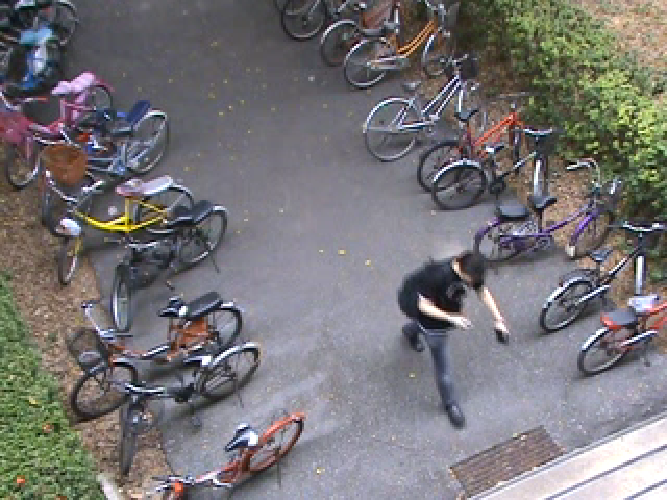
\includegraphics[width=0.2\textwidth]{figures/example-behavior01.pdf}\label{fig:example-of-scene}}
%DIFDELCMD <   %%%
\DIFdel{\hspace{0.05in}
  }%DIFDELCMD < \subfloat[]{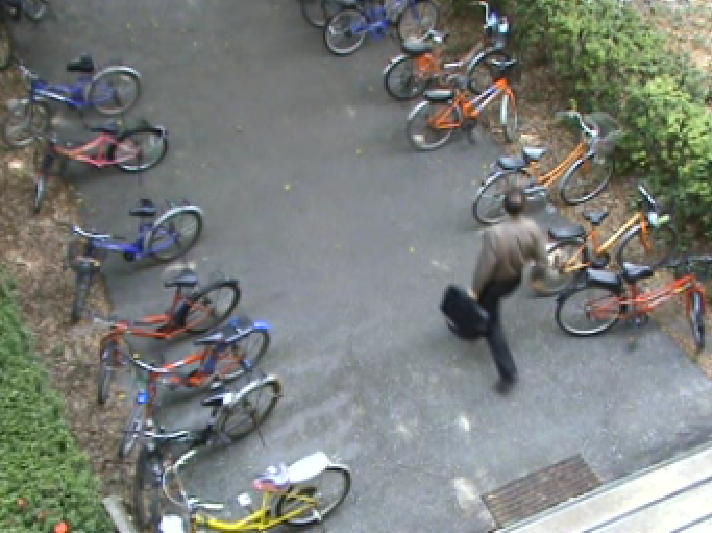
\includegraphics[width=0.2\textwidth]{figures/example-behavior02.pdf}}
%DIFDELCMD <   %%%
\DIFdel{\hspace{0.05in}
  }%DIFDELCMD < \subfloat[]{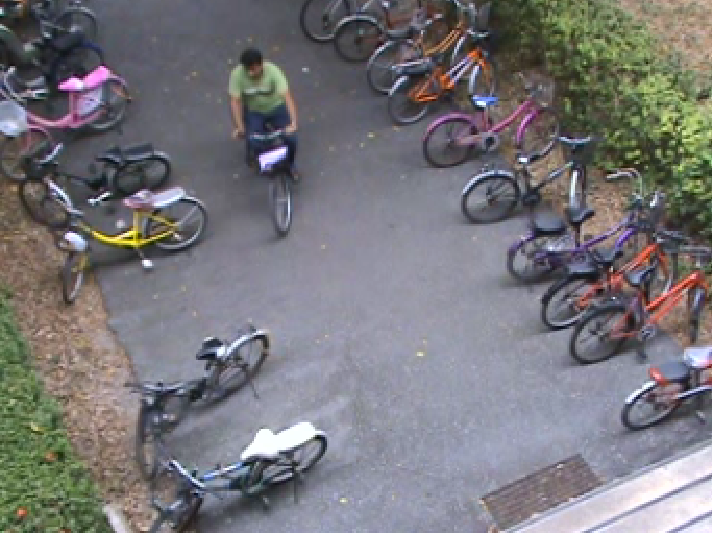
\includegraphics[width=0.2\textwidth]{figures/example-behavior03.pdf}}
%DIFDELCMD <   %%%
\DIFdel{\hspace{0.05in}
  }%DIFDELCMD < \subfloat[]{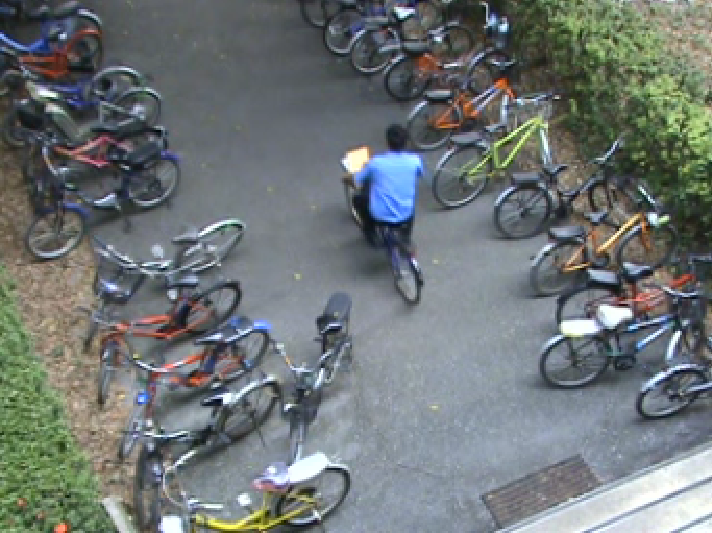
\includegraphics[width=0.2\textwidth]{figures/example-behavior04.pdf}}
%DIFDELCMD <   %%%
%DIFDELCMD < \caption[Examples of common human activities in our testbed
%DIFDELCMD <     scene.]{%
{%DIFAUXCMD
%DIFDELCMD < \small %%%
\DIFdel{Examples of common human activities in our testbed
    scene.  (a) Walking in. (b) Walking out. (c) Cycling in. (d)
    Cycling out.}}
  %DIFAUXCMD
%DIFDELCMD < \label{fig:example-behavior}
%DIFDELCMD < \end{figure}
%DIFDELCMD < %%%
\DIFdelend %DIF > \begin{figure}[t]
%DIF >   \centering
%DIF >   \subfloat[]{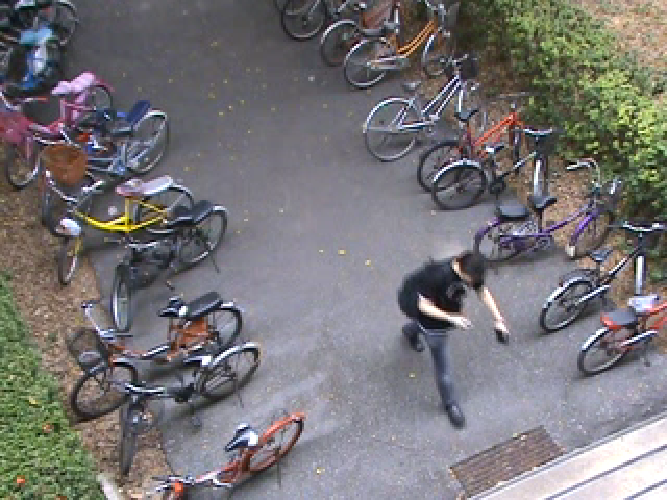
\includegraphics[width=0.2\textwidth]{figures/example-behavior01.pdf}\label{fig:example-of-scene}}
%DIF >   \hspace{0.05in}
%DIF >   \subfloat[]{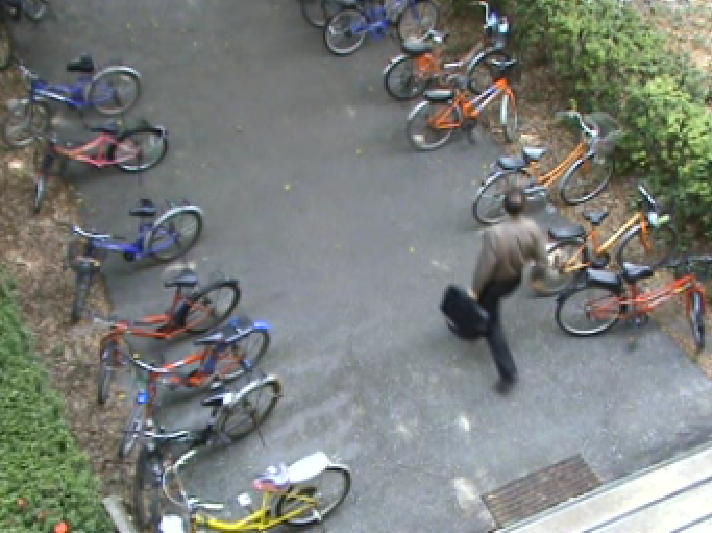
\includegraphics[width=0.2\textwidth]{figures/example-behavior02.pdf}}
%DIF >   \hspace{0.05in}
%DIF >   \subfloat[]{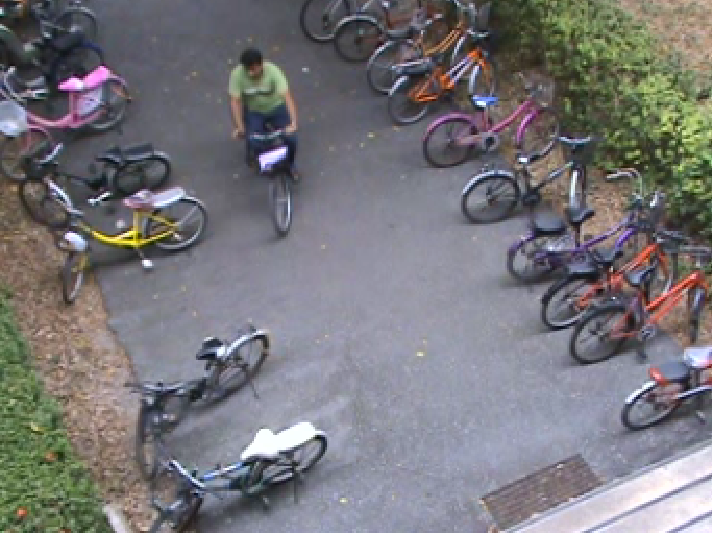
\includegraphics[width=0.2\textwidth]{figures/example-behavior03.pdf}}
%DIF >   \hspace{0.05in}
%DIF >   \subfloat[]{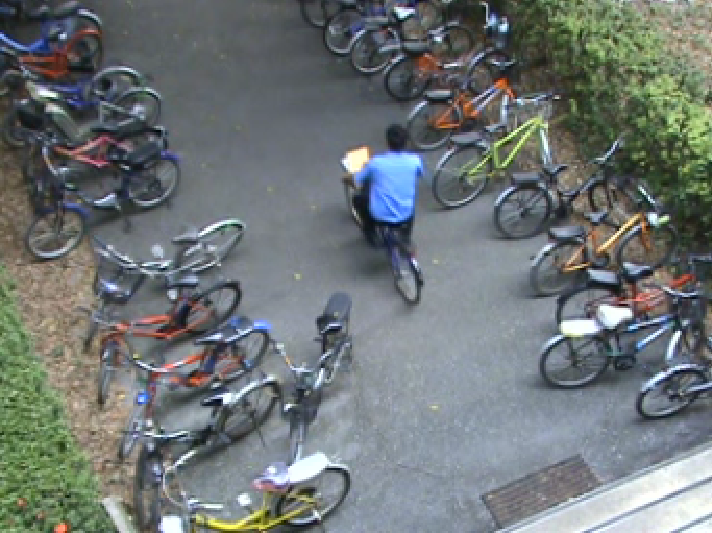
\includegraphics[width=0.2\textwidth]{figures/example-behavior04.pdf}}
%DIF >   \caption[Examples of common human activities in our testbed
%DIF >     scene.]{\small Examples of common human activities in our testbed
%DIF >     scene.  (a) Walking in. (b) Walking out. (c) Cycling in. (d)
%DIF >     Cycling out.}
%DIF >   \label{fig:example-behavior}
%DIF > \end{figure}

We performed experiments in three parts: model configuration selection
(finding an optimal set of HMMs to model the bootstrap set), anomaly
detection based on the HMM bootstrap set, and anomaly detection with
incremental learning.

\subsection{Model Configuration Selection}
\label{incremental-model-selection}

Towards model identification, we performed five-fold cross validation
with different bootstrap parameter settings and selected the
configuration with the highest accuracy in separating the normal
sequences from the abnormal sequences on the bootstrap set, as
measured by the false positive rate for abnormal sequences over all
cross validation test folds. (Every bootstrap cluster containing an
abnormal sequence is considered abnormal, so we always obtain 100\%
detection on the bootstrap set; the only discriminating factor is the
false positive rate.) The set of parameters that we varied were 1) the
number of states in each bootstrap HMM (3--8), 2) the number of
symbols/$k$-means clusters (3--8), and 3) the number $N_c$ of deviant
patterns allowed in a bootstrap cluster (1--10). To find the
distribution (parameters $\mu_c$ and $\sigma_c$) of the
per-observation log likelihood for a particular HMM, we always
generated 1,000 sequences of average length (the average length was
computed over the bootstrap set; it was 205 observations in our
experiment). For the rejection threshold $p_c$, we used a
$z$-threshold of 2.0 (i.e., $p_c = \mu_c - 2\sigma_c$), corresponding
to a Type I error rate (probability of misclassifying a sequence
generated by the HMM as not generated by the HMM) of 0.0228.

The setting of the $z$-score threshold is important. With a $z$-score
of 2, on different runs, we find that the method generates 15--30
clusters from our bootstrap set, usually perfectly classifies the
bootstrap set, and performs well on the test set. With a lower
threshold (0.5 to 1.5), only extremely similar series are clustered
together, leading to a large number of clusters and a large number of
false positives on typical behaviors that vary only slightly from what
has been seen in the bootstrap set. With higher thresholds (2.5 to 3),
patterns that are quite dissimilar get clustered, oftentimes leading
to very few clusters that do not cleanly separate the bootstrap set
and have low accuracy on the test set.

To reduce the variance in the measured false positive rate due to
random initialization, we ran the entire cross validation procedure
three times and averaged the results.

\begin{table}[t]
  \caption[Example human behavior pattern bootstrapping
    results.]{\small Example human behavior pattern bootstrapping
    results. We used linear HMMs with five states and seven
    symbols. The model consists of 17 clusters. ``W'' means ``walk''
    and ``C'' means ``cycle.'' For the six clusters containing more
    than one sequence, shown is the distribution of the patterns in
    the cluster over the activities.  The last row shows the
    distribution of the 11 clusters containing only a single sequence
    over the activity categories.}
  \begin{center}
    \begin{tabular}{c|c|c|c|c|c}
      \hline
      Cluster \# & W-in & W-out & C-in & C-out & Other \\
      \hline \hline
      1 & 44 & 0  & 20 & 0  & 0 \\ \hline
      2 & 0  & 38 & 0  & 24 & 0 \\ \hline
      3 & 0  & 0  & 3  & 0  & 0 \\ \hline
      4 & 0  & 0  & 2  & 0  & 0 \\ \hline
      5 & 0  & 0  & 0  & 0  & 6 \\ \hline
      6 & 0  & 0  & 0  & 0  & 2 \\ \hline
      One-seq clusters & 0 & 1 & 6 & 1 & 3 \\ \hline
    \end{tabular}
  \end{center}
  \label{tab:bootstrapping-results}
\end{table}

Based on the false positive rate criterion described above, we
selected the model configuration consisting of five states, seven
symbols, and $N_c = 6$ and trained a new HMM ensemble on all 150
bootstrap sequences.  We repeated the training process several times
until we obtained a model that \DIFdelbegin \DIFdel{obtained perfect accuracy }\DIFdelend \DIFaddbegin \DIFadd{perfectly maps anomalous and typical 
sequences to different clusters }\DIFaddend on the bootstrap set.  
Table \ref{tab:bootstrapping-results} shows the
distribution of bootstrap sequences across this model's 17 behavior
clusters. We used this model with the remaining 510 sequences in the
anomaly detection experiments.

\subsection{Anomaly Detection (Batch Processing)}
\label{incremental-against-global-method}

Here we evaluate the ability of our anomaly detection method to
identify anomalous events in the data not included in the bootstrap
set. Since the main concern in video surveillance is to detect every
unusual event while minimizing the false positive rate, we calculate
an ROC curve and select the detection threshold yielding the best
false positive rate at a 100\% hit rate. We reported preliminary
results for the proposed method compared to traditional machine
learning algorithms in Chapter~\ref{ch:batch}.

%a conference paper
%\shortcite{kan12detection}.

In this experiment, we compare the proposed method against HMM-based
methods using alternative representations and scoring methods similar
to those of \shortciteA{xiang08incremental}. This allows us to
determine the extent to which different event representations (our
local representation or Xiang and Gong's global representation) and
different scoring methods (our $z$-scoring method or the standard
likelihood ratio test (LRT)) contribute to anomaly detection
performance on our test set. The four methods are as follows:

\begin{enumerate}
  \item Method I: The proposed method.
  \item Method II: The proposed method, but using Xiang and Gong's
    likelihood ratio test \shortcite{xiang08incremental} rather than
    our $z$-scored likelihood method.
  \item Method III: An HMM-based method using a global event
    representation similar to that of Xiang and Gong , with our
    $z$-scored likelihood method.
  \item Method IV: The global method (Method III) using Xiang and
    Gong's likelihood ratio test rather than our $z$-scored likelihood
    method.
\end{enumerate}

%Testing methods II--IV together with our method allows us to determine
%the extent to which different event representations (our local
%representation or Xiang and Gong's global representation) and
%different scoring methods (our z-scoring method or the likelihood
%ratio test) contribute to anomaly detection performance on our test
%set. 

\DIFdelbegin %DIFDELCMD < \begin{figure}[t]
%DIFDELCMD <   \centering
%DIFDELCMD <   \begin{tabular}{ccccc}
%DIFDELCMD <     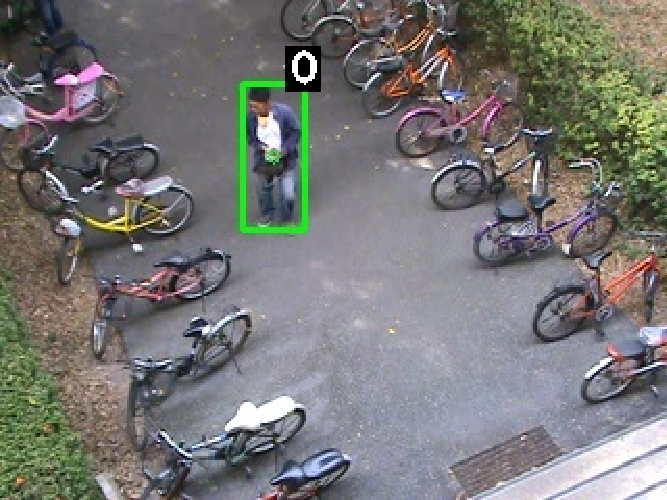
\includegraphics[scale=0.21]{figures/case-1-suspicious-0187} &
%DIFDELCMD <     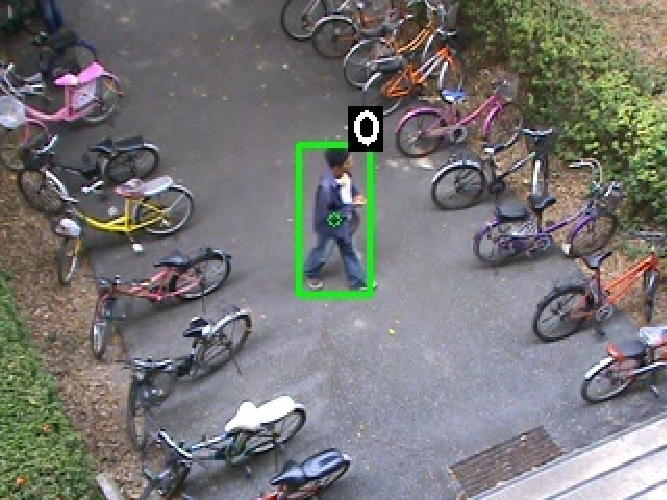
\includegraphics[scale=0.21]{figures/case-1-suspicious-0208} &
%DIFDELCMD <     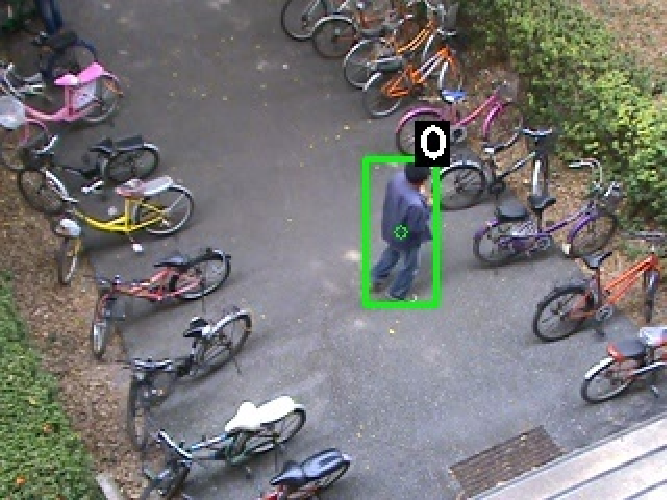
\includegraphics[scale=0.21]{figures/case-1-suspicious-0225} &
%DIFDELCMD <     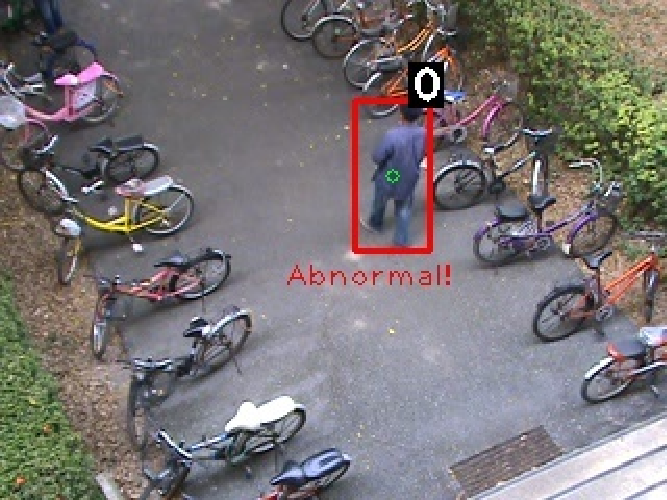
\includegraphics[scale=0.21]{figures/case-1-suspicious-0249} &
%DIFDELCMD <     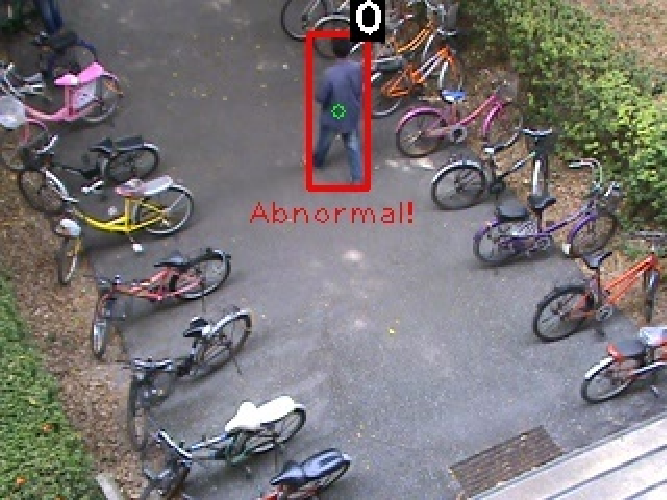
\includegraphics[scale=0.21]{figures/case-1-suspicious-0267}
%DIFDELCMD <     \\
%DIFDELCMD <     \small %%%
\DIFdel{Frame 187 }%DIFDELCMD < & 
%DIFDELCMD <     \small %%%
\DIFdel{Frame 208 }%DIFDELCMD < & 
%DIFDELCMD <     \small %%%
\DIFdel{Frame 225 }%DIFDELCMD < & 
%DIFDELCMD <     \small %%%
\DIFdel{Frame 249 }%DIFDELCMD < & 
%DIFDELCMD <     \small %%%
\DIFdel{Frame 267
  }%DIFDELCMD < \end{tabular}
%DIFDELCMD <   %%%
%DIFDELCMD < \caption[Example anomaly detected by the proposed method (Method
%DIFDELCMD <     I).]{%
{%DIFAUXCMD
%DIFDELCMD < \small %%%
\DIFdel{Example anomaly detected by the proposed method
    (Method I). The sequence contains a person walking around looking
    for an unlocked bicycle.}}
  %DIFAUXCMD
%DIFDELCMD < \label{fig:suspicious-behavior-detected}
%DIFDELCMD < \end{figure}
%DIFDELCMD < %%%
\DIFdelend %DIF > \begin{figure}[t]
%DIF >   \centering
%DIF >   \begin{tabular}{ccccc}
%DIF >     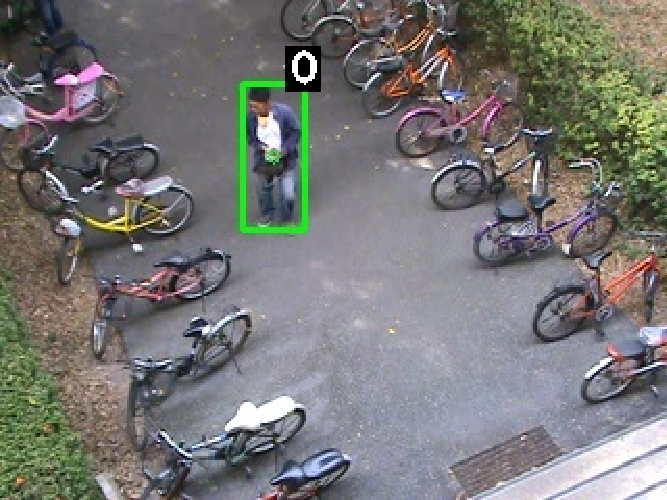
\includegraphics[scale=0.21]{figures/case-1-suspicious-0187} &
%DIF >     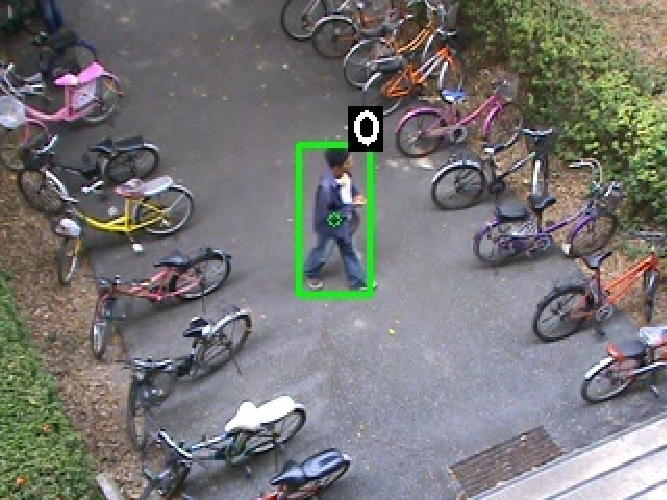
\includegraphics[scale=0.21]{figures/case-1-suspicious-0208} &
%DIF >     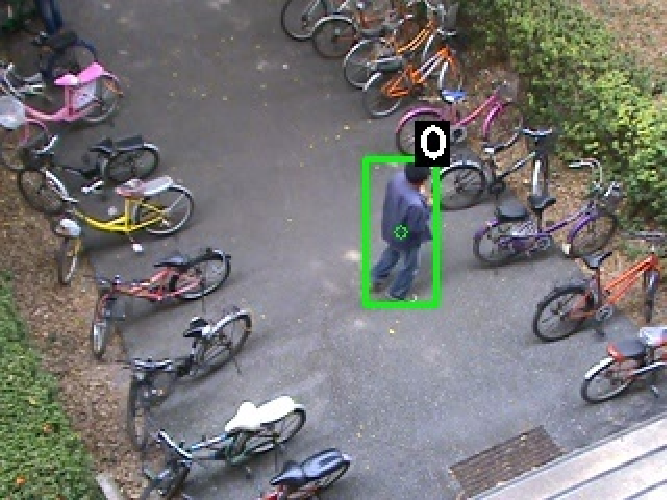
\includegraphics[scale=0.21]{figures/case-1-suspicious-0225} &
%DIF >     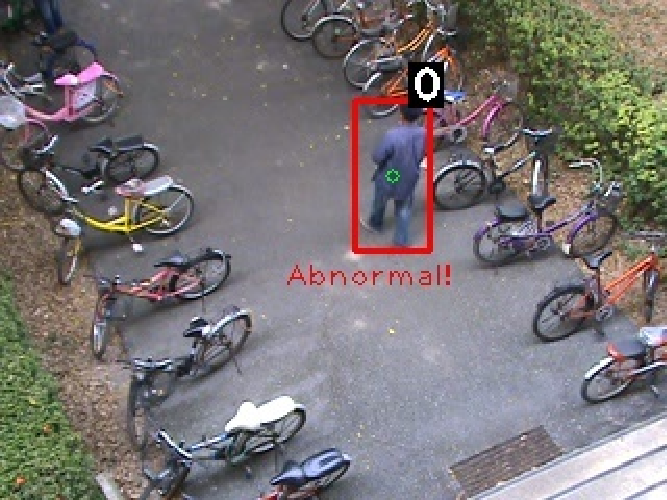
\includegraphics[scale=0.21]{figures/case-1-suspicious-0249} &
%DIF >     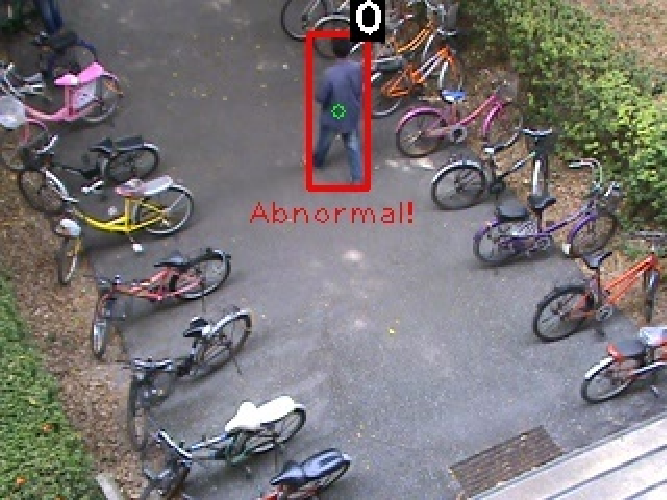
\includegraphics[scale=0.21]{figures/case-1-suspicious-0267}
%DIF >     \\
%DIF >     \small Frame 187 & 
%DIF >     \small Frame 208 & 
%DIF >     \small Frame 225 & 
%DIF >     \small Frame 249 & 
%DIF >     \small Frame 267
%DIF >   \end{tabular}
%DIF >   \caption[Example anomaly detected by the proposed method (Method
%DIF >     I).]{\small Example anomaly detected by the proposed method
%DIF >     (Method I). The sequence contains a person walking around looking
%DIF >     for an unlocked bicycle.}
%DIF >   \label{fig:suspicious-behavior-detected}
%DIF > \end{figure}

For method I and II, we used the 150-sequence bootstrap sequence set
from Section \ref{incremental-model-selection} as training data and
tested on the remaining 510
sequences. Figure \ref{fig:suspicious-behavior-detected} shows an
example of a sequence classified as abnormal.  When evaluating methods
III and IV, we extract global features rather than individual blob
features. The local method considers the single blob motion at a time,
whereas the global method simultaneously considers multiple blobs
appearing at the same time. The data set for the global method
comprises 401 sequences (366 negatives and 35 positives). We used the
first 150 sequences (139 negatives and 11 positives) for the bootstrap
set and the remaining 251 sequences (227 negatives and 24 positives)
for the test set. In all four conditions, we performed a separate
five-fold cross validation to select the best model configuration as
described in Section \ref{incremental-model-selection}.

\begin{figure}[t]
  \centering
  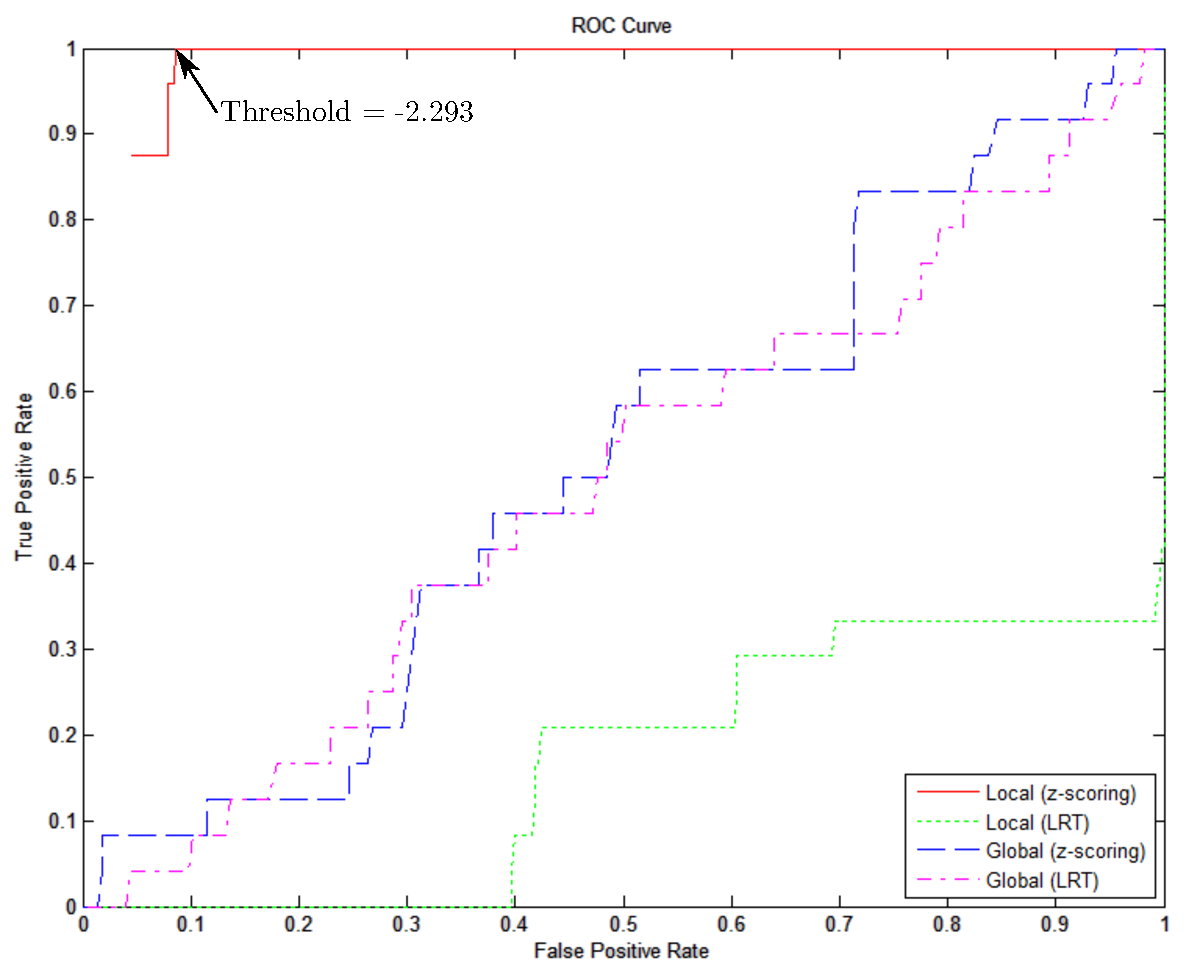
\includegraphics[width=0.8\linewidth]{figures/roc-ours-vs-global-results}
  \caption[Anomaly detection ROC curves. Solid red, dotted green,
    dashed blue, and dash-dot magenta lines represent ROCs for methods
    I, II, III, and IV, respectively.]{\small Anomaly detection ROC
    curves. Solid red, dotted green, dashed blue, and dash-dot magenta
    lines represent ROCs for methods I, II, III, and IV,
    respectively.}
  \label{fig:roc-ours-vs-global-results}
\end{figure}

\begin{table}[t]
  \caption[Anomaly detection results for the local method with the
    $z$-scoring method and the likelihood ratio test, and the global
    method with the $z$-scoring method and likelihood ratio
    test.]{\small Anomaly detection results for the local method with
    the $z$-scoring method and the likelihood ratio test, and the
    global method with the $z$-scoring method and likelihood ratio
    test. TP, FP, TN, and FN are the number of true \DIFdelbeginFL \DIFdelFL{positive}\DIFdelendFL \DIFaddbeginFL \DIFaddFL{positives}\DIFaddendFL , 
    false \DIFdelbeginFL \DIFdelFL{positive}\DIFdelendFL \DIFaddbeginFL \DIFaddFL{positives}\DIFaddendFL , true \DIFdelbeginFL \DIFdelFL{negative}\DIFdelendFL \DIFaddbeginFL \DIFaddFL{negatives}\DIFaddendFL , and false \DIFdelbeginFL \DIFdelFL{negative}\DIFdelendFL \DIFaddbeginFL \DIFaddFL{negatives}\DIFaddendFL , respectively. 
    TPR and FPR stand for true positive rate and false positive rate, 
    respectively.}
  \begin{center}
    \begin{tabular}{c|c|c|c|c|c|c}
      \hline Batch method & TP & FP & TN & FN & TPR & FPR \\ \hline \hline
      Local ($z$-scoring) & 24 & 42 & 444 & 0 & 1 & 0.086 \\ \hline
      Local (LRT) & 24 & 486 & 0 & 0 & 1 & 1 \\ \hline 
      Global ($z$-scoring) & 24 & 217 & 10 & 0 & 1 & 0.956 \\ \hline 
      Global (LRT) & 24 & 223 & 4 & 0 & 1 & 0.982 \\ \hline
    \end{tabular}
  \end{center}
  \label{tab:hmm-based-detection-results}
\end{table} 

Figure \ref{fig:roc-ours-vs-global-results} shows ROC curves for
methods I--IV.  The solid red line represents the ROC curve for method
I as we vary the threshold ($z$-score or likelihood ratio) at which a
sequence is considered anomalous. Note that the ROC does not intersect
the point $(0, 0)$ because any sequence that is most likely under one
of the HMMs modeling anomalous sequences in the bootstrap set is
automatically classified as anomalous regardless of the threshold. The
ROC reveals that a $z$-score per-observation log likelihood $\theta_z$
of $-2.293$ achieves zero false negatives at a false alarm rate of
0.086. The dotted green line is the ROC curve for method II, the
dashed blue line represents method III, and the dash-dot magenta line
represents method IV.  Table
\ref{tab:hmm-based-detection-results} shows the detailed performance
of each detection method at 100\% hit rate.

The ROC curves and FP rates show that our method clearly outperforms
the other three methods, but there is also a surprising interaction:
for the global method, $z$-scored likelihood and LRT are equally
effective, but for our local event based method, $z$-scoring is much
more effective than the LRT.  This may reflect that the LRT's use of a
mixture model is less appropriate for the local method than the global
method.

The reason that the local method is better than the global method
(albeit when combined with $z$-scoring of the likelihood) is that many
of the abnormal sequences in the test set tend to be locally similar
to the abnormal sequences in the bootstrap set but globally
different. The local method treats concurrent but spatially separate
local events as being independent, whereas the global method attempts
to construct a joint model over the entire scene.  The global method
might be improved with a larger bootstrap set.

%For example, a person is
%looking for an unlocked bicycle while another person is leaving a
%building. The local method considers the former event as anomalous;
%the latter event as normal. Whereas, the global method considers it as
%only one anomalous event.

The log likelihood ratio test fails to detect completely new anomalous
patterns when the pattern has a very low likelihood according to the
abnormal model and the normal model but has a slightly higher
likelihood according to the normal model. In order for the LRT test to
detect such patterns, we need to adjust the LR threshold, causing
higher false positives (increasing the number of false positives to
about 30--40).  Since our approach creates a new abnormal model for
any low-likelihood observation, regardless of the relative likelihood,
it does not suffer from this problem.

\subsection{Anomaly Detection with Incremental Learning}

In this experiment, we evaluate the use of incremental HMM learning
for anomaly detection. We used the same settings and model
configuration as in the batch method experiments described in Section
\ref{incremental-against-global-method}.  Since we incorporate a completely
new observation sequence at each increment, the likelihood over all
the sequences may increase or decrease. In the current work, we
reestimate $\mu_c$ and $\sigma_c$ after every update by generating
1,000 new sample sequences.  The update process could obviously be
optimized.

Overall results of incremental learning are shown in Table
\ref{tab:iml-detection-results}. Compared to the batch method, the
incremental version of the proposed method (local method with
$z$-scoring) obtains a nearly four-fold decrease in the false positive
rate (2.2\% vs.\ 8.6\%) at the cost of a 9\% decrease in the hit rate.
The results shown in the table are based on a fixed $z$-score
threshold of $\theta_z=2.0$.  To better enable comparison of the
results for batch and incremental learning, we varied $\theta_z$ to
obtain false positive rates at 100\% detection rates and to obtain
equal error rates (EERs). The incremental method achieves a 3.7\%
false alarm rate at a 100\% hit rate, compared to 8.6\% for the batch
method.  It achieves an EER of 95.8\%, compared to 91.8\% for the
batch method.

Overall, these results demonstrate that the incremental algorithm
detects anomalies more effectively with lower false alarm rates.  It
is better able than the batch method to learn new forms of normal
behavior.  New behavior classes are always called anomalous at first,
so completely new behaviors (suspicious or not) will always trigger a
false positive and lead to the creation of a new model trained on the
new sequence.  These one-sequence HMMs tend to generate sequences with
very low variance in the log likelihood. Such models do not often get
updated with new sequences, but they do from time to time. In this
experiment, new sequences were assigned to existing multi-sequence
HMMs 466 times, existing single-sequence HMMs 44 times, and were used
to create new sequences 5 times.  The improvement in performance of
the incremental method over the batch method thus comes first from
tuning the parameters of the existing behavior classes (both typical
and anomalous), but it also comes from the use of additional typical
labels for the false positive anomalous series.

\begin{figure}[t]
  \centering
  \subfloat[]{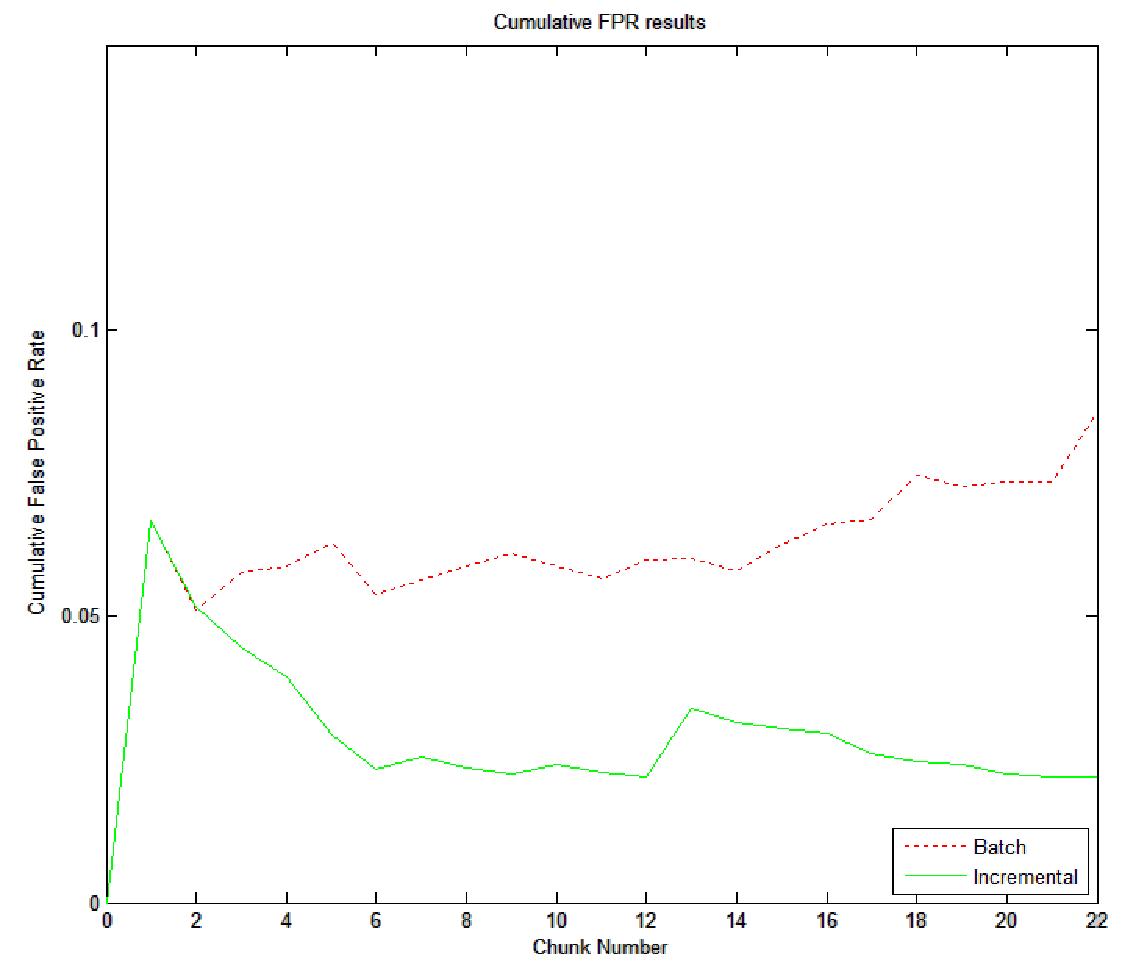
\includegraphics[width=3in]{figures/cFPR-chunk-results-5-trials.pdf}}
  \subfloat[]{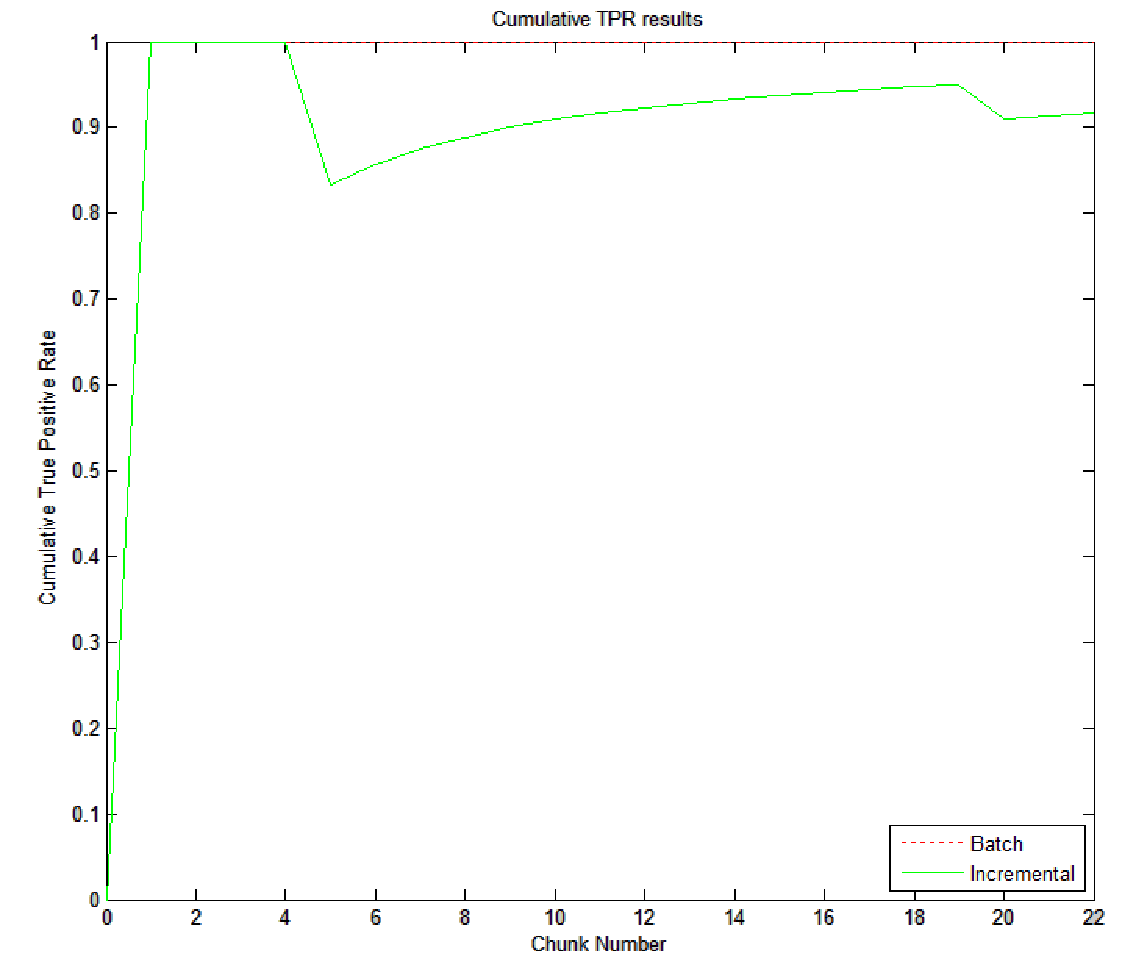
\includegraphics[width=3in]{figures/cTPR-chunk-results-5-trials.pdf}}
  \caption[Comparison of batch learning and incremental learning over
    time.]{\small Comparison of batch learning (dotted red line) and
    incremental learning (solid green line) over time.  (a) Cumulative
    false positive rates. (b) Cumulative true positive rates.  Each
    point is an average of the false positive or true positive rates
    over 5 trials.}
  \label{fig:chunking-results}
\end{figure}

To further understand the performance differences between the batch
and incremental methods, we partitioned the test data sequentially
into chunks and computed the false and true positive rates for each
chunk of observations.  Initially, we set the chunk size to 10. If our
system detects a suspicious pattern within a chunk, we record it and
compute the false positive rate for the chunk. If the method does not
detect any suspicious pattern, on the other hand, we increase the
chunk's size by 1 until a true positive is given, then we reset the
next chunk's size back to 10. This resulted in 22 chunks for our test
set. Cumulative false and true positive rate data are shown in
Figure \ref{fig:chunking-results}. Initially, the incremental
method has the same false alarm rate as the batch method.  However,
the incremental method's false alarm rate drops quickly to achieve the
eventual 2.2\% false alarm rate at a 91\% hit rate.

\begin{table}[t]
  \caption[Anomaly detection results on average for incremental HMM
    learning for our local method and the global method over 5
    trials.]{\small Anomaly detection results on average for
    incremental HMM learning for our local method and the global
    method over 5 trials. TP, FP, TN, and FN are the number of true positive, 
    false positive, true negative, and false negative, respectively. 
    TPR and FPR stand for true positive rate and false positive rate, 
    respectively.}
  \begin{center}
    \begin{tabular}{c|c|c|c|c|c|c}
      \hline
      Incremental method & TP & FP & TN & FN & TPR & FPR \\
      \hline \hline
      Local ($z$-scoring) & 21.8 & 9.8  & 476.2  & 2.2 & 0.91 & 0.022 \\ \hline
      Local (LRT) & 16 & 243.4 & 212.6 & 8 & 0.6664 & 0.564 \\ \hline
      Global ($z$-scoring)  & 3 & 13 & 214 & 21 & 0.125 & 0.057 \\ \hline
      Global (LRT)  & 18 & 184.4 & 42.6 & 6 & 0.75 & 0.813 \\ \hline
    \end{tabular}
  \end{center}
  \label{tab:iml-detection-results}
\end{table}

For comparison, we also tested incremental versions of the three
alternative approaches previously described in Section
\ref{incremental-against-global-method}: local method with LRT, global method
with $z$-scoring, and global method with LRT. In every condition, we
used the same model configuration and detection threshold found best
in the batch experiment.  For our incremental approach, both typical
and atypical behavior models get updated during incremental learning.
The results are shown in Table \ref{tab:iml-detection-results}.
Similar to the incremental method results, none of the three alternative
methods performed as well as the proposed method. Our experimental
results also demonstrate that over 510 new patterns, our approach
requires security personnel to correct the system a mere 9--10 times.

The incremental version of the global method has lower false alarm
rates and lower detection rates than the batch version of the global
method. To an extent, the fixed $z$-score threshold of 2.0 places the
global method at an inopportune position on the ROC curve. However,
generally, we find that the global method with $z$-scoring performs
poorly regardless of the threshold. With the global representation,
the abnormal models tend to be quite specific whereas the normal
models tend to be a little more general, so that we often see new
anomalous patterns receiving relatively good scores from some normal
models but no good scores from abnormal models. The anomalies thus
tend to get incorrectly classified as normal more often.

Besides improved detection, another advantage of our incremental
approach is that it is more efficient than the batch method over time.
To demonstrate this, we performed a brief experiment on the runtime
requirements on a Core 2 Duo processor at 2.2 GHz. We first trained a
model with 1,000 synthetic sequences then re-trained that model with
1,000 sequences plus 10 new sequences using batch learning or
incremental learning. The batch method required 33816 ms, whereas our
incremental method with only the 10 new sequences required only 1056
ms. Obviously, the incremental approach uses far less time than the
batch method to integrate new data into the training set, because it
does not require retraining on old data.

As a final manipulation, we performed a brief experiment to determine
whether incremental learning alone without a bootstrap set is
effective on these data.  We found that test set performance improves
with the size of the bootstrap set.  With more bootstrap data we tend
to discover more compact behavior classes, leading to better
performance on incremental updates. Conversely, incremental updates
without a good bootstrap model lead to poor detection rates throughout
the experiment. So while a no-bootstrap method could lessen the user's
up-front workload, we conclude that the risk of missed anomalies is
too high.

\section{Discussion}
\label{incremental-conclusion}

We have proposed and evaluated an efficient method for bootstrapping
scene-specific anomalous human behavior detection systems that
incrementally learns behavior models without requiring storage of
large databases of training data. The method requires minimal
involvement of a human operator; the only required action is to label
the patterns in a small bootstrap set as normal or anomalous and then
to label false positive alarms as normal when they occur.

On a testbed data set acquired in a real-world video
surveillance situation, with a bootstrap set of 150 sequences,
the incremental method achieves a false positive rate of 2.2\% at a
91\% hit rate.  With threshold tuning, the method can yield an equal
error rate of 95.8\% or a false positive rate of 3.7\% at a 100\% hit
rate. The experiments show that it is possible to learn a complex set
of varied behaviors occurring in a specific scene with a collection of
simple HMMs while allowing evolution of the learned typical behavior
model over time.  This can lead in turn to more effective anomaly
detection.

\FloatBarrier




%%% --- Maybe use later ---

%%% WE MAY USE THIS INFO %%%
%For Method V, the dash-dot magenta line in
%\figurename~\ref{fig:roc-results} represents the ROC curve for the
%global method as we vary the likelihood threshold at which a sequence
%is considered anomalous. We found that our local approach performs
%better than the global approach on our small dataset. The performance
%of the global method is shown in Table
%\ref{tab:detection-results}. Since the global approach aims to model
%the whole scene, it may perform better with more training data
%covering all possible typical activities in a scene.

% remove the comparison with the ML algorithms due to limitied length
% --- beginning of the comparison with the ML algorithms ---
% \subsubsection{Comparison with Traditional Machine Learning Algorithms}
% 
% In this experiment, we apply the proposed method and traditional
% machine learning algorithms ($k$-nearest neighbors, Mahalanobis
% classification, and support vector machines) to the same problem.
% Since the main concern in video surveillance is to detect every
% unusual event while minimizing the false positive rate, in every
% experiment except $k$-NN, we calculate an ROC curve and select the
% detection threshold yielding the best false positive rate at a 100\%
% hit rate. ($k$-NN does not have a detection threshold.) Our
% experimental hypothesis was that the proposed method for modeling
% scene-specific behavior patterns should obtain better false positive
% rates than the traditional methods.
% 
% \begin{figure}[t]
%   \begin{center}
%     \begin{tabular}{ccccc}
%       \includegraphics[scale=0.21]{suspicious-behavior-0187.pdf} &
%       \includegraphics[scale=0.21]{suspicious-behavior-0208.pdf} &
%       \includegraphics[scale=0.21]{suspicious-behavior-0225.pdf} &
%       \includegraphics[scale=0.21]{suspicious-behavior-0249.pdf} &
%       \includegraphics[scale=0.21]{suspicious-behavior-0267.pdf}
%       \\
%       Frame 187 & Frame 208 & Frame 225 & Frame 249 & Frame 267
%     \end{tabular}
%   \end{center}
%   \caption{Example anomaly detected by the proposed method (Method
%     I). The sequence contains a person walking around looking for an
%     unlocked bicycle.}
%   \label{fig:suspicious-behavior-detected}
% \end{figure}
% 
% \paragraph{Proposed method} We used the 150-sequence bootstrap
% sequence set from Section \ref{sec:model-selection} as training data
% and tested on the remaining 510 sequences.
% \figurename~\ref{fig:suspicious-behavior-detected} shows an example of
% a sequence classified as abnormal.
% 
% \paragraph{$k$-NN} We used the same division into training and test data as
% our proposed method. For the distance measure, we used the same DTW
% distance measure used in our hierarchical clustering method. We varied
% $k$ from 1 to 5 and retained the best result.
% 
% \paragraph{Mahalanobis classifier} We used the 139 typical
% sequences in the bootstrap set for training and used all abnormal
% sequences (including the abnormal sequences in the bootsrap set) for
% testing. To get a fixed-dimension measurement vector for each
% sequence, we calculated a summary vector consisting of the means and
% standard deviations of each observation vector element over the entire
% sequence. With seven features in the observation vector, we obtained a
% 14-element vector summarizing each sequence then $z$-score normalized
% each component of the summary vector. Since we are performing
% probability density estimation for the normal patterns, we applied PCA
% to the 139 normal sequences in the bootstrap set.  We chose the number
% of principal components accounting for 80\% of the variance in the
% bootstrap data. Finally, we classified the remaining 521 test
% sequences using the PCA model to calculate the Mahalanobis distance of
% each sequence's summary vector to the mean of the normal bootstrap
% patterns' summary vectors.
% 
% \paragraph{SVMs} We used the same summary vector technique used for
% Mahalanobis classifier but performed supervised classification using
% support vector machines. We used the radial basis function kernel
% implementation in LIBSVM \cite{CC01a} with grid search for the optimal
% hyperparameters using five-fold cross validation on the training set
% (150 sequences).
% 
% \begin{figure}[t]
%   \begin{center}
%     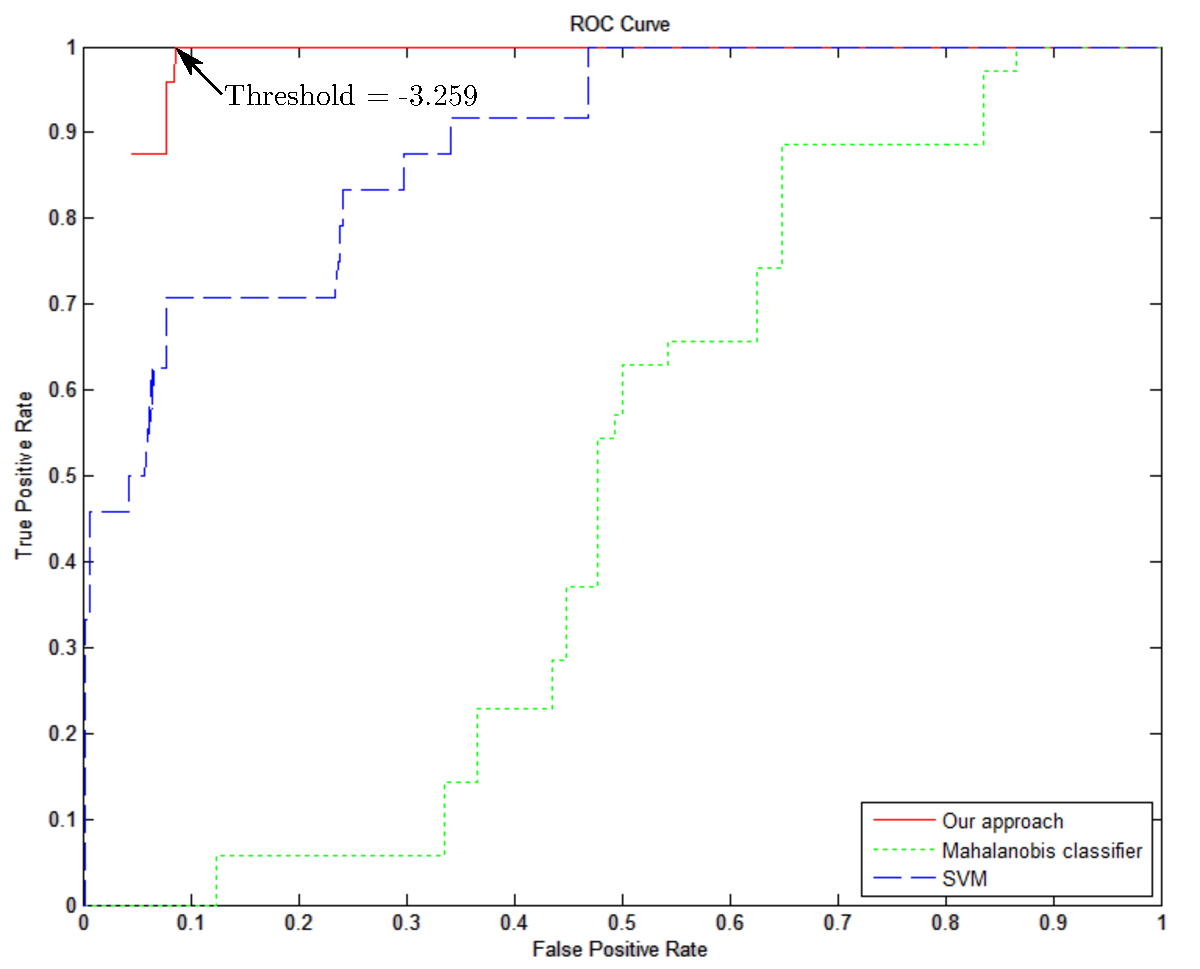
\includegraphics[width=3in]{figures/roc-ours-vs-ml-results.pdf}
%   \end{center}
%   \caption{Anomaly detection ROC curves. The proposed method
%     outperforms the Mahalanobis and SVM classifiers.}
%   \label{fig:roc-ours-vs-ml-results}
% \end{figure}
% 
% \begin{table}[t]
%   \begin{center}
%     \begin{tabular}{ | c | c | c | c | c | c | c | }
%       \hline
%       Method                 & TP & FP  & TN  & FN & TPR   & FPR \\
%       \hline\hline
%       Proposed method        & 24 & 42  & 444 & 0  & 1     & 0.086 \\ \hline
%       $k$-NN ($k$ = 1)       & 19 & 1   & 485 & 5  & 0.792 & 0.002 \\ \hline
%       Mahalanobis classifier & 35 & 421 & 65  & 0  & 1     & 0.866 \\ \hline
%       SVM                    & 24 & 228 & 258 & 0  & 1     & 0.469 \\ \hline
%     \end{tabular}
%   \end{center}
%   \caption{Anomaly detection results for the proposed method, $k$-NN,
%     Mahalanobis classifier, and SVM, respectively. For the Mahalanobis
%     classifier, we include 11 abnormal sequences from the bootstrap
%     set in the test set, so the total number of positives is 35.}
%   \label{tab:detection-results}
% \end{table}
% 
% \paragraph{Results}
% \figurename~\ref{fig:roc-ours-vs-ml-results} shows the anomaly
% detection results in the form of ROC curves for our proposed method,
% Mahalanobis classifier, and SVM.  The solid red line represents the
% ROC curve for our method as we vary the likelihood threshold at which
% a sequence is considered anomalous.  Note that the ROC does not
% intersect the point $(0, 0)$ because any sequence that is most likely
% under one of the HMMs modeling anomalous sequences in the bootstrap
% set is automatically classified as anomalous regardless of the
% threshold. The ROC reveals that a $z$-score threshold of $-2.293$
% achieves zero false negatives at a false alarm rate of 0.086.  The
% dotted green line is the ROC curve for Mahalanobis classifier,
% obtained by varying the Mahalanobis distance threshold, and the dashed
% blue line is the ROC curve for the SVM, obtained by varying the
% threshold on the signed distance to the separating hyperplane used for
% classification as normal or abnormal.
% 
% Table~\ref{tab:detection-results} shows the detailed performance of
% the best models with 100\% hit rate for our method, Mahalanobis, and
% SVM, as well as the $k$-NN model with the best hit rate.  The high
% false positive rate of the Mahalanobis and SVM methods at the 100\%
% hit rate threshold as well as the the overall poor performance in the
% ROC analysis show that the Mahalanobis classifier and SVMs are clearly
% inferior to our proposed method.  While $k$-NN's false positive rates
% are much lower than those obtained in our method, the hit rates are
% unacceptable.
% --- end of the comparision with the ML algorithms ---


%%% MAYBE USEFUL TEXT %%%

%(a person walking around looking for an unlocked bicycle).

% \begin{table}[t]
%   \begin{center}
%     \begin{tabular}{ | c | c | c | c | c | c | }
%       \hline
%       TP & FP & TN & FN & TPR & FPR \\
%       \hline\hline
%       24 & 36 & 450 & 0 & 1 & 0.074 \\ \hline
%     \end{tabular}
%   \end{center}
%   \caption{Anomaly detection results at 100\% hit rate for the
%     proposed method in Experiment I.}
%   \label{tab:detection-results}
% \end{table}

%Since PCA requires a fixed-length input vector, we calculated, for
%each sequence in the testbed data set, a summary vector consisting of
%the means and standard deviations of each observation vector element
%over the entire sequence. 

% \begin{table}[t]
%   \begin{center}
%     \begin{tabular}{ | c | c | c | c | c | c | }
%       \hline
%       TP & FP & TN & FN & TPR & FPR \\
%       \hline\hline
%       35 & 421 & 65 & 0 & 1 & 0.87 \\ \hline
%     \end{tabular}
%   \end{center}
%   \caption{PCA anomaly detection results in Experiment III. We include 
%   11 abnormal sequences from the bootstrap set in the test set, so the
%   total number of positives is 35.}
%   \label{tab:pca-detection-results}
% \end{table}

% \begin{table}[t]
%   \begin{center}
%     \begin{tabular}{ | c | c | c | c | c | c | }
%       \hline
%       TP & FP & TN & FN & TPR & FPR \\
%       \hline\hline
%       24 & 228 & 258 & 0 & 1 & 0.469 \\ \hline
%     \end{tabular}
%   \end{center}
%   \caption{SVM anomaly detection results in Experiment IV.}
%   \label{tab:svm-detection-results}
% \end{table}

%Although the results are clearly better than those obtained from
%$k$-NN or PCA, they are also clearly inferior to those obtained in
%Experiment I.

%\ifnum\short=0 For $k$-NN to be a
%practical anomaly detection method, we would have to adjust it.  For
%example, we could impose a distance threshold beyond which a pattern
%is considered anomalous even if a majority of the nearest neighbors
%are normal. \fi

% \begin{table}[t]
%   \begin{center}
%     \begin{tabular}{ | c | c | c | c | c | c | c | }
%       \hline
%       $k$ & TP & FP & TN & FN & TPR & FPR \\
%       \hline\hline
%       1 & 19 & 1 & 485 & 5 & 0.792 & 0.002 \\ \hline
%       2 & 19 & 2 & 484 & 5 & 0.792 & 0.004 \\ \hline
%       3 & 16 & 0 & 486 & 8 & 0.667 & 0 \\ \hline
%       4 & 16 & 1 & 485 & 8 & 0.667 & 0.002 \\ \hline
%       5 & 14 & 0 & 486 & 10 & 0.583 & 0 \\ \hline
%     \end{tabular}
%   \end{center}
%   \caption{$k$-NN anomaly detection results in Experiment II.}
%   \label{tab:kNN-results}
% \end{table}

%      $k$-NN ($k$ = 2) & 19 & 2 & 484 & 5 & 0.792 & 0.004 \\ \hline
%      $k$-NN ($k$ = 3) & 16 & 0 & 486 & 8 & 0.667 & 0 \\ \hline
%      $k$-NN ($k$ = 4) & 16 & 1 & 485 & 8 & 0.667 & 0.002 \\ \hline
%      $k$-NN ($k$ = 5) & 14 & 0 & 486 & 10 & 0.583 & 0 \\ \hline
%      Proposed incremental method & 23.9 & 13.6 & 472.4 & 0.067 &
%      0.997 & 0.028 \\ \hline
